\chapter[The ILC]{The future of high-energy physics: the International Linear Collider}
\label{chap:ILC}

\newacronym{LHC}{LHC}{Large Hadron Collider}
\newacronym{ILD}{ILD}{International Large Detector}
\newacronym{ILC}{ILC}{International Linear Collider}
\newacronym{CLIC}{CLIC}{Compact LInear Collider}
\newacronym{SRF}{SRF}{Superconducting Radio-Frequency}
 %Introduction on the limits of the \gls{LHC} and why a new colliding experiment is needed
 % First part: describing the main characteristics of the ILC (energy scale, legnth, luminosity)
 %   -> Design (e+/e- sources, damping ring, main linacs, beam delivery system and interaction region )
 %   -> Beam properties
 %   -> Background: beam-beam interaction (luminosity enhancement ~2 BUT hard bremstrahlung that degrades the energy spectrum), pair background (coherent and incoherent production of e+e-)
 % Second part: Detector
 %   -> Option for two experiments (PUSH-PULL)
 %   -> Main differences between the \gls{ILD} and the SiD
 %   -> Talking about the \gls{ILD} (VTX, SIT, TPC, f)

  Since 2008, the \gls{LHC} is actually the most powerful tool in high energy physics to have a better understanding of the universe, particularly with the discovery in 2012 of a new particle compatible to the boson predicted by the spontaneous symmetry breaking of the SM \cite{Aad2012, Chatrchyan2012}.
  Although the \gls{LHC} is an impressive machine able to reach the highest energy scales of collisions available on Earth with a centre-of-mass energy of 14 TeV, the complex environment of the events generated hides the access to some fundamental parameters. 
  To achieve more precise measurements of the Higgs boson, but also to test the validity of the SM and other physics theories introduce in the chapter \ref{chap:SM}, the high energy physics community has merged on the necessity to build a linear electron-positron collider, that will work as a complementary accelerator to the \gls{LHC}.
  
  This chapter will explain the motivations to invest a huge amount of money in a new great world project. It will present the complementary nature of the lepton and hadron colliders and the main advantages of the lepton collisions will be discussed.
  After giving an overview of the ILC with its basic design and the experiment models, we will focus on the design of one of the experiments: the \gls{ILD}.

 \minitoc
  
  \section{To a linear lepton collider}
 
 % Before to introduce the ILC machine and explain the reasons to invest in such a project, I will give an overview of the \gls{LHC} abilities and the limits of this giant machine.
  The most impressive accelerator ever built is located at CERN in Geneva, Switzerland. 
  It is the world largest particle accelerator, with a circumference ring of nearly 27 kilometers, straddling the Swiss and French borders.
  It is designed to collide two counter rotating beams of protons or heavy ions, with a possibility to reach centre-of-mass energies of 14 TeV with a high peak luminosity of $10^{34} \text{ cm}^2 \text{s}^{-1}$.
  The goals of the \gls{LHC} are to perform further tests on the SM, search for new forces or produce dark matter candidates. 
  Indeed, the collider covers a wide energy range at the constituent level while running at a fixed beam energy.
  Unfortunately, the measurements can not reach the highest precision.
  
  Complementary to a discovery machine such as the \gls{LHC}, a machine to perform precise measurement should be built: the lepton collider.

    \subsection{Advantages of a linear lepton collider}
    
    First of all, during each collision at an hadron collider, only a part of the total centre-of-mass energy is available for the process evolved, so the initial four-vector momentum is not known. 
    By colliding leptons, which are structureless objects, the full centre-of-mass energy is available for the elementary process. 
    The initial four-vector momentum of an interaction is exactly known, hence the event can be fully reconstructed.

    Secondly, with a lepton collider, the beam energy is tunable and both electron and positron beams can be polarised. 
    The selection of an appropriate polarisation can boost the signal and suppress the background cross-section. 

    Thirdly, as seen on the first point, at the \gls{LHC}, only a fraction of the partons are contributing to the interesting process. 
    The proton-proton interaction cross section is dominated by inelastic background QCD processes.
    The signal event is then accompanied by large backgrounds produced by the interaction of other partons collisions.
    This background has an impact on the detector design (high radiation tolerance and selective trigger implementation) and masks the elementary process of interests. 
    The lepton colliders do not suffer from this kind of background and at similar energies, the event rate is lower as those of hadron colliders.
    Moreover, the interaction of electrons and positrons is purely electroweak.
    So, the detectors do not have to handle extreme data rates and they can be used without any trigger.
    This will allow to get a better sensitivity to any possible signature of new physics.

    This main advantages of the lepton colliders do not explain the choice of a linear collider to perform fine and precise measurements.
    The reason of that choice is provided by the equation \ref{eq:Esynchrotron} describing the synchrotron radiation emitted by a particle moving in a circular accelerator.
    
    \begin{equation}
     E = ....
       \label{eq:Esynchrotron}
    \end{equation} 

    The radiative energy loss is proportional to the radius, the energy of the particle and its mass.
    To compensate that loss, a circular electron-positron accelerator should have an extremely big raidus. 

    \todo{Write energy loss, may be if it is E4/rm4}


    To reach the same energy scale at a linear collider, it requires a bigger number of accelerating cavities and would be bigger than a circular collider.
    Indeed, in a circular collider, th particle bunches are being accelerated many time in the ring up to reach the energy of collision.
    Unfortunately, the track of particles are bended, leading to an energy lose through synchrotron radiation.
    The energy loss is proportional to the particle's energy
    

    % - Leptons are structureless -> Well known 4-vector momentum to reconstruct fully the event
    % - Quarks are made of partons => Impossible to know exactly the 4-vector momentum
    % - Partons that do not participate to the collisions contribute to parisitic soft interaction (QCD bg)
    %       => Hide elementary processes (small polar angle)
    %       => Needs implementation of trigger
    % - Beam energy tunable and polarisation of e+/e- can enhance the signal and suppress the background cross-section 
    
    % LINEAR VS CIRCULAR COLLIDER!
    \subsection{Future linear lepton collider}

    As it was mentioned before, the precise measurements offered by lepton collider is one of the key point to constraint the limits of the \gls{SM} and to characterise precisely all the known particles.
    Since the 1980's, several linear collider technologies have been developed, leading in the 1990's to five major accelerator technologies: \gls{SRF}, the \gls{CLIC} technology and three different normal conducting technologies (S-band, C-band and X-band).
    At the beginning of the 2000's, a committee for the future linear collider was formed and has chosen in 2004 the \gls{SRF} technology and all the efforts were done in that direction to build the \gls{ILC}\todo{Paper on ILC}.
    The technology used for that future experiment are also used for the XFEL at DESY and at KEK in Japan.
    An other linear collider project led by the CERN is being prepared: the \gls{CLIC}.
    It has a more challenging technology to aim a nominal energy of 3 TeV.
    Contrary to the \gls{ILC}, \gls{CLIC} plans to use radio-frequency structures and a two beam concept\todo{Paper on CLIC}. 
    An other plan not reasonably practicable would be to develop a muon collider instead of electron-positron collider.
    This project is more tricky than the two other ones.
    Even if the muons are not suffering from the synchrotron radiation due to their mass and make possible to build a circular collider, their life-time makes the acceleration more challenging.

    For the purpose of this thesis, let's drop the \gls{CLIC} and muon collider to focus in details on the \gls{ILC}.
     
   % Several projects are being discussed for the next experimentation: the \gls{ILC}\todo{Paper on ILC}, \gls{CLIC}\todo{Paper on CLIC} and a muon collider. 
   % The first project features a more mature technology than the two others. 
   % Indeed, the linear collider technologies have been developed since the 1980's, leading to 5 major accelerator technologies: superconducting RF, S-, C- and X-band normal conducting technologies and the CLIC technology.
   % But in 2004, a committee has chosen the superconducting technology and all the efforts were done in that direction.
   % Also, this technology is already used for the XFEL experiment at DESY.
   % \gls{CLIC} has a major challenging technology and aims a nominal energy of 3 TeV. 
   % Instead of using superconducting RF, it will use RF structures and a two-beam concept.
   % The muon collider is also one possibility but more tricky.
   % Even if the muons are not suffering from the synchrotron radiation, allowing to build a circular collider, the life time of this particles makes the acceleration more challenging.

  \section{The ILC machine}
  
    The ILC should be the next lepton collider experiment and will be situated in Japan.
    During 2016, the final site where the experiment will be hold is going to be decided.
    The most likely site candidate is located in the north of Japan, in the region of Kitakami. 
    
    \subsection{Baseline design}

   \begin{figure}
      \centering
      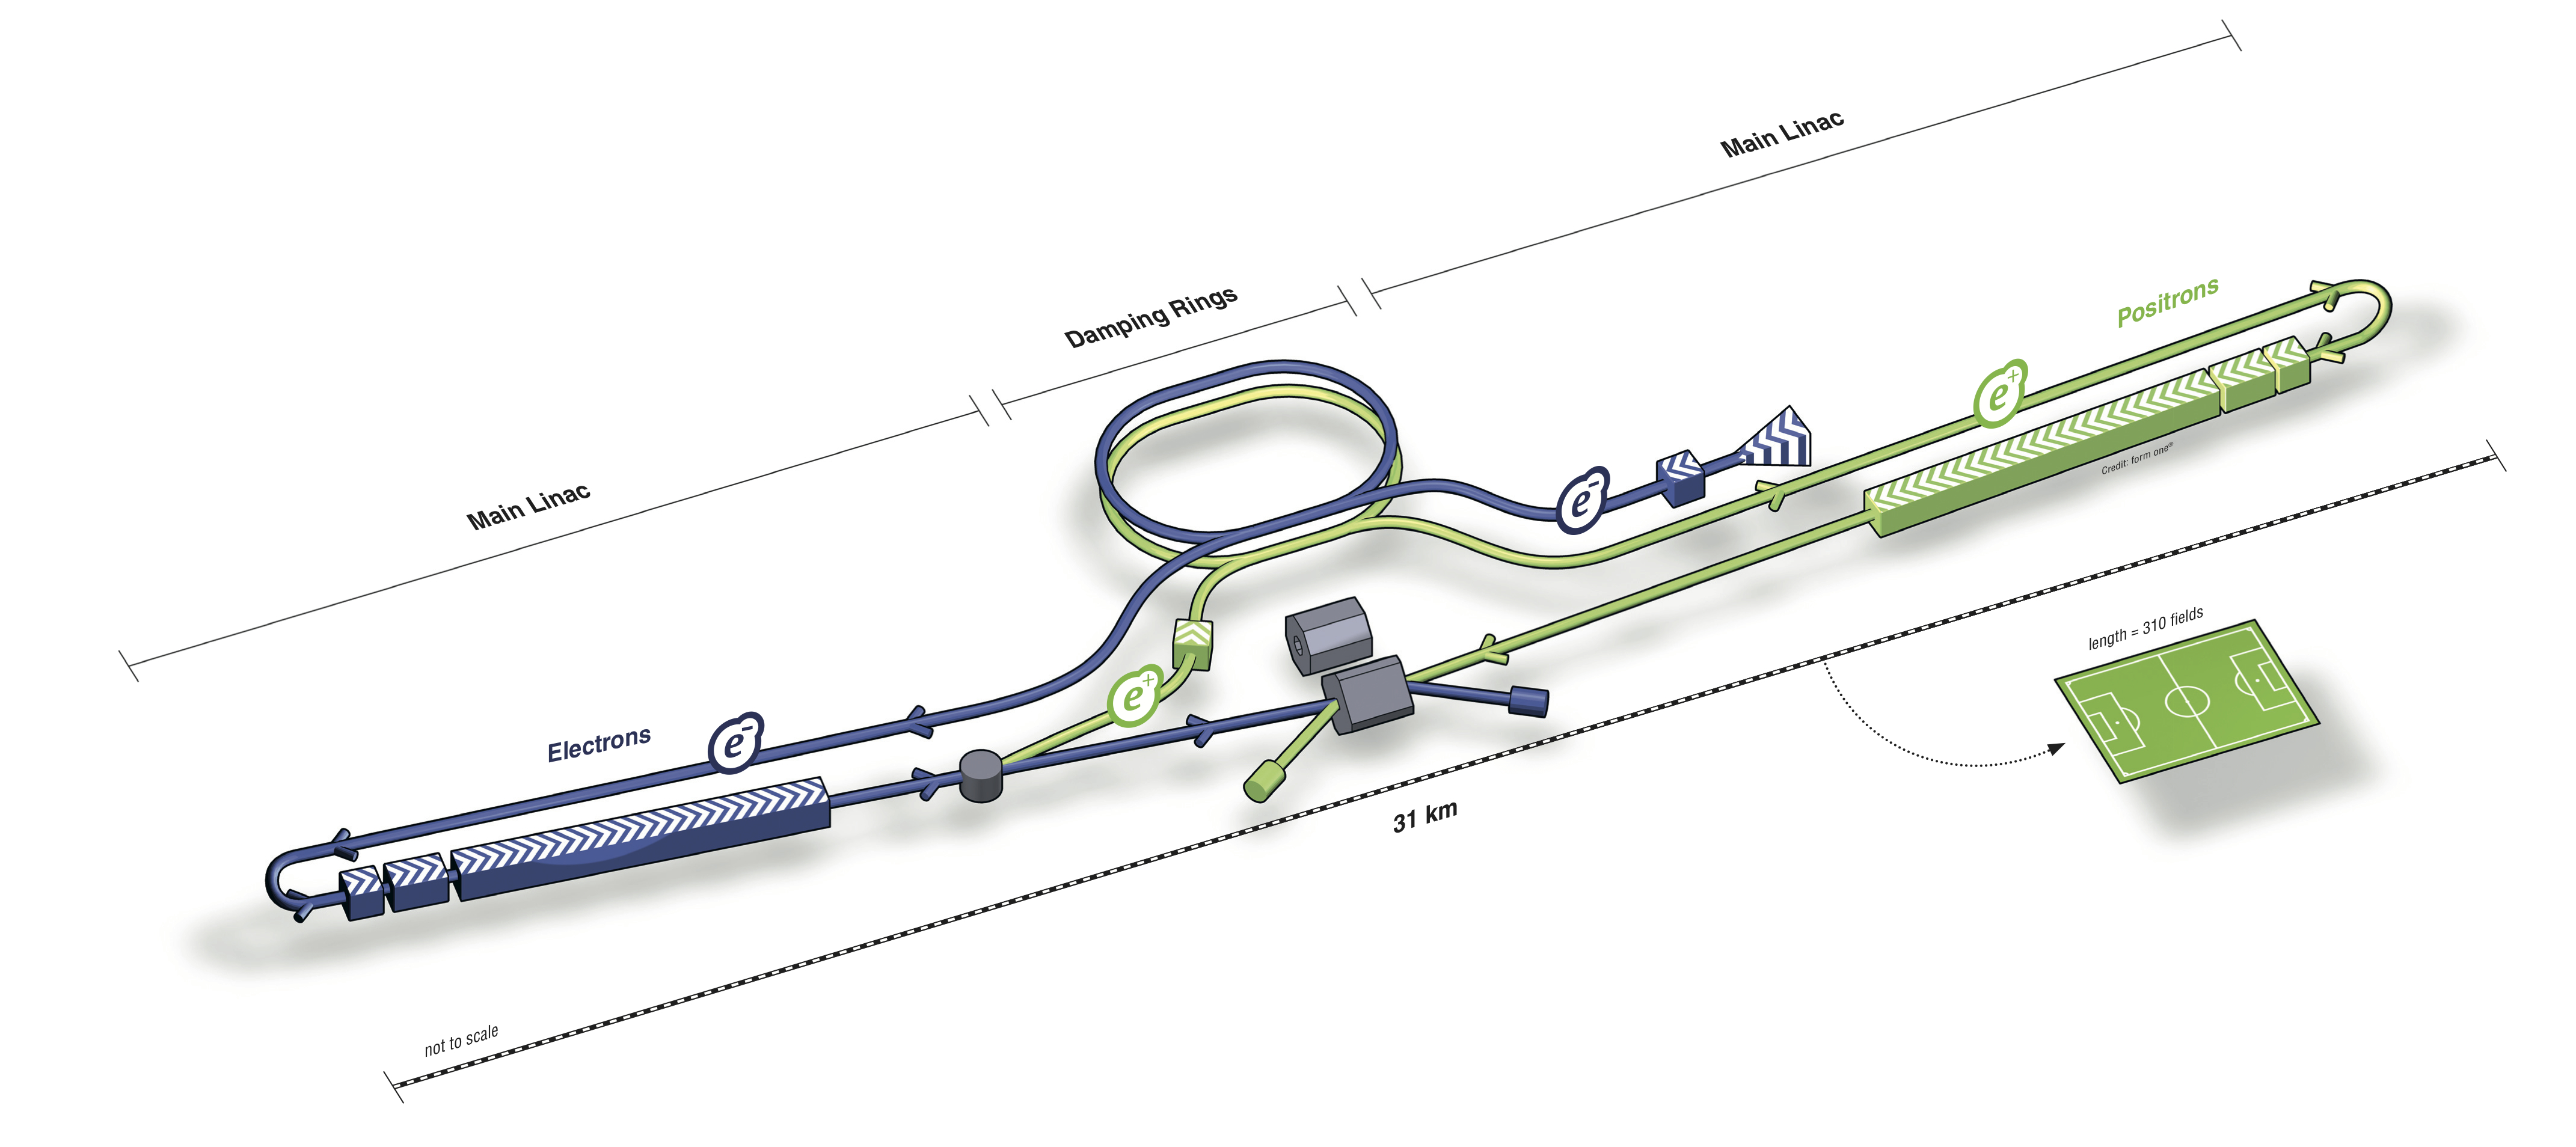
\includegraphics[width = 15 cm]{Pictures/ILC}
      \caption{Basic design of the International Linear Collider}
      \label{fig:ILC}
    \end{figure}


    The ILC is planed to collide electrons an positrons at a center-of-mass energy up to 500 GeV, with energy variability down to 200 GeV for 31 kilometers long accelerator. 
    An upgrade to reach the centre-of-mass energy of 1 TeV is also possible, but the accelerator should be extended to achieve a total length of 50 kilometers.
    It is designed to generate a total of $500 \text{fb}^{-1}$ of data during the first four years of operation. The luminosity will reach a peak of $2 \times 10^{34}\text{cm}^{-2}\text{s}^{-1}$ at $\sqrt(s) = 500 \text{GeV}$.

    The main components of the ILC are the electrons and positrons sources, the damping ring, the main LINAC, the Beam Delivery System (BDS) and the interaction region. Two experiments will participate and will share the same interaction region. Via a push-pull system, the detector will be alternatively positioned and running, while the other one would be maintain in a cavern next to the interaction region. 

    \subsection{Beam parameters}

    The polarised electrons are produced by a laser firing a photocathode in a DC gun.
    The electrons are then pre-accelerate to 76 MeV thanks to non-superconducting accelerating structures.
    Then, they are injected into a 250 m long superconducting linac to reach the energy of 5 GeV.

    

    \begin{figure}
      \centering
      \missingfigure{Bunch structure}
      \caption{Bunch structure of the ILC: ...}
      \label{fig:bunches}
    \end{figure}

    \subsection{Background}

  \section{The ILC detectors concept}

    \subsection{Overview of the two experiments}
    
  Although the ILC is a linear collider with only one beam line, two experiments will participate.
  The duplication of the beam to get two permanent fixed detectors is too expensive and difficult to built.
  Instead, the collaboration has the idea to have only one interaction point.
  A push/pull system will allow to change the detector 

  Two detector designed with complementary features have been developed. 
  Their designs will reach the ILC precision measurements and search for new physics. 
  They are optimised for the particle flow algorithm (PFA) to measure the final states with high accuracy.
  This leads to a high hermeticity, high granular calorimeters and excellent tracking and vertexing. 
  The two experiments are the Silicon Detector (SiD) and the International Large Detector (\gls{ILD}) and a global comparison of the two detectors is going to be presented on the next subsection.

      \subsection{SiD VS ILD}
    \begin{figure}
      \centering
      \missingfigure{ILD concept and SiD concept}
      \caption{The ILC detectors concept: on the left, a design of the SiD, on right a design of the ILD }
      \label{fig:SiLD}
    \end{figure}    
    
    \subsection{The ILD detector}
    
    \begin{figure}
      \centering
      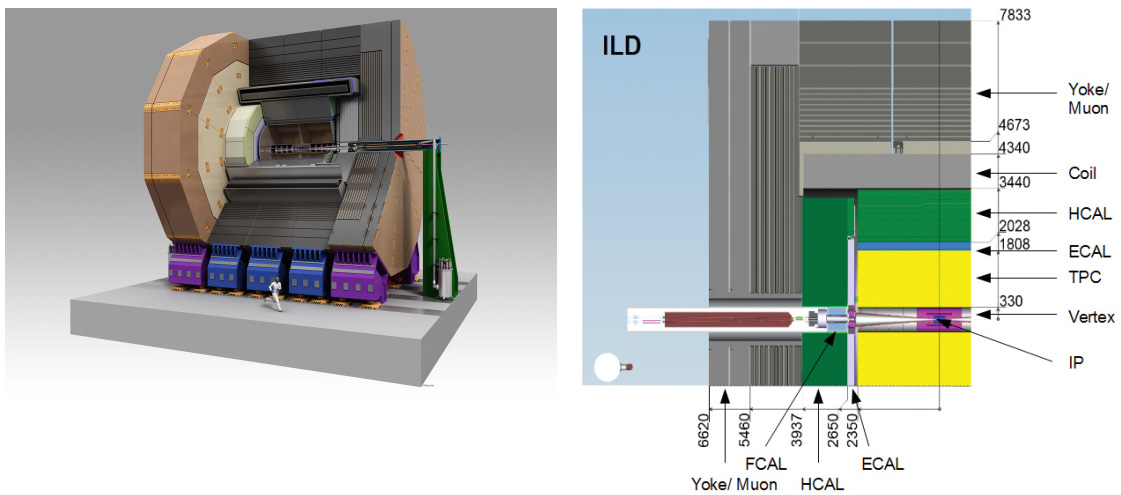
\includegraphics[width = 20cm]{Pictures/ild-detector-ilc.jpg}
      \caption{The ILD detector concept with its subdetector system}
      \label{fig:ILD}
    \end{figure}

    The \gls{ILD} is a detector designed to follow the requirements given before.
    

      \subsubsection{Vertex detector}

      The chapter~\ref{chap:vxd} will introduce more in details the vertex detector requirements for the \gls{ILD} and the different design proposals. 
      For the moment, two designs are under study for the vertex detector.
      The first one is made of five single sided layers and the other one three double sided detection layers.
      The design of a vertex detector is driven by the material budget and the precision of the measurements.

      \subsubsection{Tracking}
      %Silicon tracking
      %TPC

      The main tracking system for the \gls{ILD} is done by the Time-Projection-Chamber (TPC).
      It is a gaseous detector with a low material budget designed to measure the particles' trajectory.
      When a particle goes through the TPC, it ionises the gas, creating electrons that are drifting to the anode thanks to a high voltage.
      The anode is the part where the readout plates are installed.
      It provides 3D position of the particles tracks thanks to the wires and the anode (give x-y) and the z coordinate is given by the drifting time.
      In addition to the exact position measurement, this detector is also able to measure the energy $\frac{dE}{dx}$ deposited by the particle and would be a first step for a particle identification.
      \todo{Rewrite description of the TPC, it is such shitty right now...}

      The requirements to design a TPC at the ILC are given by two main values: 
      
      \begin{itemize} 
        \item Single point resolution $\sigma_{s.p.}$ which should be lower than $100 \mu\text{m}$ in the $r\phi$ direction and less than $500 \mu\text{m}$ in the z direction
        \item The minimum distance to separate two hits which should be lower than 2 mm.
      \end{itemize}

      The TPC thought for the \gls{ILD} is constituted of a central barrel part, with an inner radius of $\simeq 33 \text{cm}$ and a outer radius of $\simeq 180 \text{cm}$ and two endcaps with a detection area of $10 m^2$. 
      The solid angle coverage is up to $|\cos{\theta} \simeq 0.98|$.
      The barrel will be filled with a gas mixture called T2K (3 \% of Ar-CF4 and 2 \% of isobutane).
      Due to the low material budget and the ability to cope with a high magnetic field, the TPC is compliant with a Particle FlowAlgorithm~\ref{sec:PFA} \todo{Add PFA citation}. 


      To improve the track reconstruction, the TPC is surrounded by high silicon detectors: two barrel components, the Silicon Internal Tracker (SIT) and the Silicon External Tracking (SET); an end-cap component, the End-cap Tracking Detector and the Forward Tracking Detector (FTD).
      The SIT is linking the tracking between the VXD and the TPC, whereas the SET is giving an entry point to the ECAL after the TPC.
      Both system provide precise space points and improve the overall momentum resolution.
      The goal of the SIT is to improve the momentum resolution, the reconstruction of low $p_{T}$ charged particles and the reconstruction of long lived particles.
      The coupling of the SIT and SET provide also a time stamping information.

      The ETD is located within the gap separating the TPC and the end-cap calorimeter. 
      It improves the momentum resolution for charged tracks with a reduce path in the TPC.
      It also reduces the effect of the material of the TPC end-plate. 
      The material budget of this end-plate is estimated to 15 \% of $X_0$.

      As the TPC does not provie any coverage in the forward region, seven silicon disks ensure efficient and precise tracking down to very small angles.
      The ETD and FTD make sure to get a full tracking hermeticity.

      To simplify the system layout and the maintenance, the SIT, SET and ETD are made of single sided strip layers titled by a small angle with respect to each other. 
      They are placed in a so called false double-sided layers.
      The SIT has two layers of micro-strip, instead of one layer for the SET. 
      The technology studied are micro-strip sensors with an area of $10x10 \text{cm}^2$, with a pitch of 50 $\mu$m, a thickness of 200 $\mu$m and a edgeless.
      The dead area of the sensors will be reduced down to few microns instead of 100 $\mu$m.
      The spatial point resolution aimed for this detectors is $\sim 7.0 \ \mu$m in the $r\phi$ direction.
      The table~\ref{tab:siTrackParam} gives the single point resolution aimed, as well as the angular coverage and the material budget.

      \begin{table}[!h]
        \centering
          \begin{tabular}{c c c c}
          \hline %----------------------------
          Detector &  Single point resolution ($\mu$m) &  coverage  & material budget $X_0$ (\%) \tabularnewline
          \hline %----------------------------
          \hline %----------------------------
          \multirow{2}*{SIT}  & $\sigma_{R-\phi} = 7.0 $  & \multirow{2}*{$\cos{\theta} \sim 0.91$ } & \multirow{2}*{0.65} \tabularnewline
                              & $\sigma_Z = 50.0 $ & & \tabularnewline
          SET      & $\sigma_R = 7.0$ & $\cos{\theta} \sim 0.79$ & 0.65 \tabularnewline
          ETD      & $\sigma_X = 7.0$ & $\cos{\theta} \sim 0.799 - 0.985 $ & 0.65 \tabularnewline
          \end{tabular}
          \caption{Parameters aimed for the silicon tracker using micro-strips sensors.}
          \label{tab:siTrackParam}
      \end{table}

     The FTD is placed in the forward direction, between the beam pipe and the inner field cage of the TPC, where the magnetic field becomes less and less useful to bend charged tracks and so the determination of a precise momentum is more difficult.
     It consists of seven tracking disks: the two firsts are pixel detectors to cope with expected high occupancies and the five others are strip detectors.
     The pointing resolution will vary between $3.0-6.0 \ \mu$m for the two firsts layers and $7.0 \ \mu$m for the five other ones.
     

      \todo{Check the table and values....}

      \subsubsection{Calorimeters}

      The calorimeters design is driven by the particle flow requirements.
      Each particle must be reconstructed individually in the detector with a jet energy measurement equal to:
      \begin{equation}
        \frac{\Delta E}{E} = 30 \% / \sqrt{\frac{E}{GeV}}
        \label{eq:jetRes}
      \end{equation}

      The energy resolution obtained in equation~\ref{eq:jetRes} is obtained thanks to a combination of information from the tracking system and the calorimeters. 
      The choice of technology used for the calorimeter will be determined by the pattern recognition performance. 
      One of the \gls{ILD} detector's goal is for example to be able to get a jet energy resolution sufficient to clean separate W and Z hadronic decays.
      
      The average jet energy distribution is roughly: 
      \begin{itemize}
        \item $62 \%$ of charged particles (mainly hadrons)
        \item $27 \%$ of $\gamma$
        \item $10 \%$ of long-lived neutral hadrons
        \item $1.5 \%$ of $\nu$
      \end{itemize}

      The electromagnetic calorimeter (ECAL) is the first calorimeter after the tracking system.
      Its role is to identify photons and leptons and measure their energy, nevertheless it is also the first section to develop the hadron showers.
      Its fine segmentation makes important contribution to hadron-hadron jet separation.
      For the \gls{ILD}, a compromise between the performance and the cost has led to use a sampling calorimeter realised with tungsten absorber.
      They are three options under study for the active area.
      The first one, called SiW-ECAL, is made of silicon pin diodes with a pitch of $5 \times 5 \text{mm}^2$. 
      It has the advantage to cover a large area, to be reliable and simple to operate, to have thin readout layers and can be operate in 3.5 T magnetic field.
      The second option is made of scintillator strips readout by photo-sensors and is called ScECAL.
      It has an active area of $5 \times 45 \text{mm}^2$ arranged in alternative directions to achieve an effective granularity of $5 \times 5 \text{mm}^2$ 
      The weakness of this technology happened in dense jets environment, where the reconstruction becomes more and more complicated.
      Some alternatives are also thought, like the Micromegas chambers. Nevertheless this technology is less advanced compared to the others.
      One good candidate could be the use of MAP\footnote{Monolithic Active Pixel} sensors.
      They have the advantage to get the readout on the same.... blablabla...
      and by choosing standard CMOS processes, the cost of fabrication would be reduced.

      The hadronic calorimeter (HCAL) has the role to separate the deposits energy of charged and neutral hadrons and to precisely measure the energy deposited.
      It is also a sampling calorimeter using stainless steel instead of tungsten as absorber. 
      The rigidity of stainless steel makes possible to get a self supporting structure limiting the dead areas.
      Two different options for the active medium area are studied.
      The analogue HCAL (AHCAL) is made of scintillator tiles, whereas the semi-digital options is made of gaseous devices.
      Analogue HCAL and Semi-Digital HCAL (SDHCAL)  and strong candidate: Glass Resistive Plate Chamber (GRPC)

      The calorimeter system is completed in the very forward region by three different subsystems. 
      The LumiCAL serves as luminosity monitor by measuring the Bhabha scattering $e^+e^- \rightarrow e^+e^-$ via emission of virtual $\gamma$, the BeamCal as beamstrahlungsmonitor 

      

      \subsubsection{Magnetic Field and yoke}
